\documentclass[12pt]{article}
\usepackage[a4paper, margin=1in]{geometry}
\usepackage[utf8]{inputenc}
\usepackage{hyperref}
\usepackage{textcomp}
\usepackage{listings}
\usepackage{xcolor}
\usepackage{blindtext}
\usepackage{enumitem}
\usepackage{bm}
\usepackage{courier}
\usepackage{amssymb}
\usepackage{mathtools}
\usepackage{mathrsfs,amsmath}   %The amsmath package
\definecolor{mygreen}{rgb}{0,0.6,0}
\definecolor{mygray}{rgb}{0.5,0.5,0.5}
\definecolor{mymauve}{rgb}{0.58,0,0.82}

\DeclareMathSizes{10}{10}{10}{10}

\lstset{ %
  backgroundcolor=\color{white},   % choose the background color; you must add \usepackage{color} or \usepackage{xcolor}
  basicstyle=\footnotesize,        % the size of the fonts that are used for the code
  breakatwhitespace=true,         % sets if automatic breaks should only happen at whitespace
  breaklines=true,                 % sets automatic line breaking
  captionpos=b,                    % sets the caption-position to bottom
  commentstyle=\color{mygreen},    % comment style
  deletekeywords={...},            % if you want to delete keywords from the given language
  escapeinside={\%*}{*)},          % if you want to add LaTeX within your code
  extendedchars=true,              % lets you use non-ASCII characters; for 8-bits encodings only, does not work with UTF-8
  frame=single,	                   % adds a frame around the code
  keepspaces=true,                 % keeps spaces in text, useful for keeping indentation of code (possibly needs columns=flexible)
  keywordstyle=\color{blue},       % keyword style
  language=Matlab,                 % the language of the code
  otherkeywords={*,...},           % if you want to add more keywords to the set
  numbers=none,                    % where to put the line-numbers; possible values are (none, left, right)
  numbersep=5pt,                   % how far the line-numbers are from the code
  numberstyle=\tiny\color{mygray}, % the style that is used for the line-numbers
  rulecolor=\color{black},         % if not set, the frame-color may be changed on line-breaks within not-black text (e.g. comments (green here))
  showspaces=false,                % show spaces everywhere adding particular underscores; it overrides 'showstringspaces'
  showstringspaces=false,          % underline spaces within strings only
  showtabs=false,                  % show tabs within strings adding particular underscores
  stepnumber=2,                    % the step between two line-numbers. If it's 1, each line will be numbered
  stringstyle=\color{mymauve},     % string literal style
  tabsize=4,	                   % sets default tabsize to 2 spaces
  title=\lstname,                   % show the filename of files included with \lstinputlisting; also try caption instead of title
  upquote=true,
}
\renewcommand{\lstlistingname}{Script}

\hypersetup{
    bookmarks=true,         % show bookmarks bar?
    unicode=false,          % non-Latin characters in Acrobat’s bookmarks
    pdftoolbar=true,        % show Acrobat’s toolbar?
    pdfmenubar=true,        % show Acrobat’s menu?
    pdffitwindow=false,     % window fit to page when opened
    pdfstartview={FitH},    % fits the width of the page to the window
    pdftitle={My title},    % title
    pdfauthor={Author},     % author
    pdfsubject={Subject},   % subject of the document
    pdfcreator={Creator},   % creator of the document
    pdfproducer={Producer}, % producer of the document
    pdfkeywords={keyword1, key2, key3}, % list of keywords
    pdfnewwindow=true,      % links in new PDF window
    colorlinks=true,       % false: boxed links; true: colored links
    linkcolor=red,          % color of internal links (change box color with linkbordercolor)
    citecolor=green,        % color of links to bibliography
    filecolor=magenta,      % color of file links
    urlcolor=cyan           % color of external links
}

\newcommand\tab[1][1cm]{\hspace*{#1}}

\newcommand{\icol}[1]{% inline column vector
  \left[\begin{smallmatrix}#1\end{smallmatrix}\right]%
}

\newcommand{\irow}[1]{% inline row vector
  \begin{smallmatrix}[#1]\end{smallmatrix}%
}

\newcommand\numberthis{\addtocounter{equation}{1}\tag{\theequation}}

\begin{document}
\title{METR7203 Problem Based Assignment 2}
\author{Callum Rohweder s4357594}
\date{August 2017}

\maketitle

\section{Question 1}
The inverted pendulum on a cart system is illustrated in figure 1. It can be seen that the coordinates of interest for this are p (linear position), and theta (the pendulum angle with respect to the upwards vertical axis). To control this system, an input F is applied on the cart, allowing it to compensate for the movement of the pendulum; altering the cart's position. 


\begin{center}
\begin{figure}[htb]
	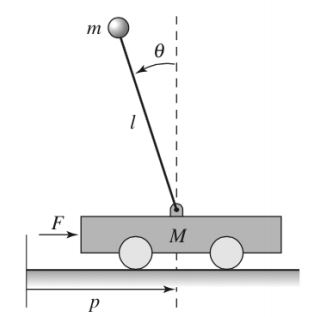
\includegraphics[width=0.8\textwidth]{mass_and_cart.jpg}
\caption{Inverted Pendulum on a cart diagram}
\end{figure}
\end{center}



//
The parameters of this system are:

\rightarrow the damping of the pendulum ($\rho$)

\rightarrow the damping of the cart ($c$)

\rightarrow the mass of the cart ($M$)

\rightarrow the mass of the pendulum as a point load ($m$) at distance (%$l$)

\rightarrow the acceleration sure to gravity ($g$)

\rightarrow the position of the cart ($p$) and derivatives ($p_{d}$, $p_{dd}$)

\rightarrow the angle of the pendulum ($th$) and derivatives ($th_{d}$, $th_{dd}$)






Using Lagranges equations, the equations of motion for this system can be expressed. 







\clearpage

\section{Question 2}
In assignment one, a block diagram model of cruise control was made using Simulink. This question is related to that model, as it is essentially a scripted version of that simulation in a function, $cruise\_control.m$, shown below. The objective in this activity was to construct a phase portrait representing the velocity and integral of the PI controller states, to show how selected initial conditions and internal functions of the controller can lead to asymptotic stability at an equilibrium; at the desired velocity.

The formulas used in calculation are represented in the matlab code, the most important equation to note is the actuator equation lambda,
\vspace{\baselineskip}

$  \lambda = \left\{
\begin{array}{11}
      0 & u\leq 0 \\
      u & 0\leq u\leq 1 \\
      1 & 1\leq u \\
\end{array} 
\right. $
\vspace{\baselineskip}

Where u is the controller output, effectively the throttle command, and lambda is the throttle actuation. In this case, 1 represents the throttle being completely on and 0 represents no throttle. Thus, the car is limited to only going forward, as $\lambda$ and the applied torque are always positive, and there is no braking system (apart from drag, friction and gravitational forces).

The controller output, u, is made from a PI controller which corrects the error between a regulation velocity $Vr$ and the actual velocity of the car body $v$. The state variables used for the phase portrait are $v$ and $z$, where $z$ is the integral state of the PI controller and thus their derivatives are the body's acceleration, $a$, and the velocity error, $e$, respectively.

Using the Simulink model from assignment 1, the following code could be produced, which computes the derivative states of inputs $[v, z]$, as per the state-space representation of the control system $x' = F(x)$

\vspace{\baselineskip}

\lstinputlisting[caption={cruise\_control.m}]{cruise_control.m}

\vspace{\baselineskip}

Following this, a script was created to plot the states in time in time, using the state-space equation results; from $cruise\_control.m$.
This was done using the ode45 function, an ODE solver which outputs the response in time. A phase-portrait is a 2D graph visualising a two states change in time, where an asymptotically stable equilibrium  point represents the two states coming to their steady state values; as time goes to infinity. Thus it is necessary to gather information on the state's values in time, and plotted on a phase portrait, which is done in the following matlab script:

\vspace{\baselineskip}

\lstinputlisting[caption={PBA2\_script.m}]{PBA2_script.m}

\vspace{\baselineskip}

The response of both states in time to an input $[v, z] = [1, 10]$ is shown in the figure below, where it can be seen that both the velocity and integral controller state reach a steady-state value within 100 seconds.

\begin{center}
\begin{figure}[htb]
	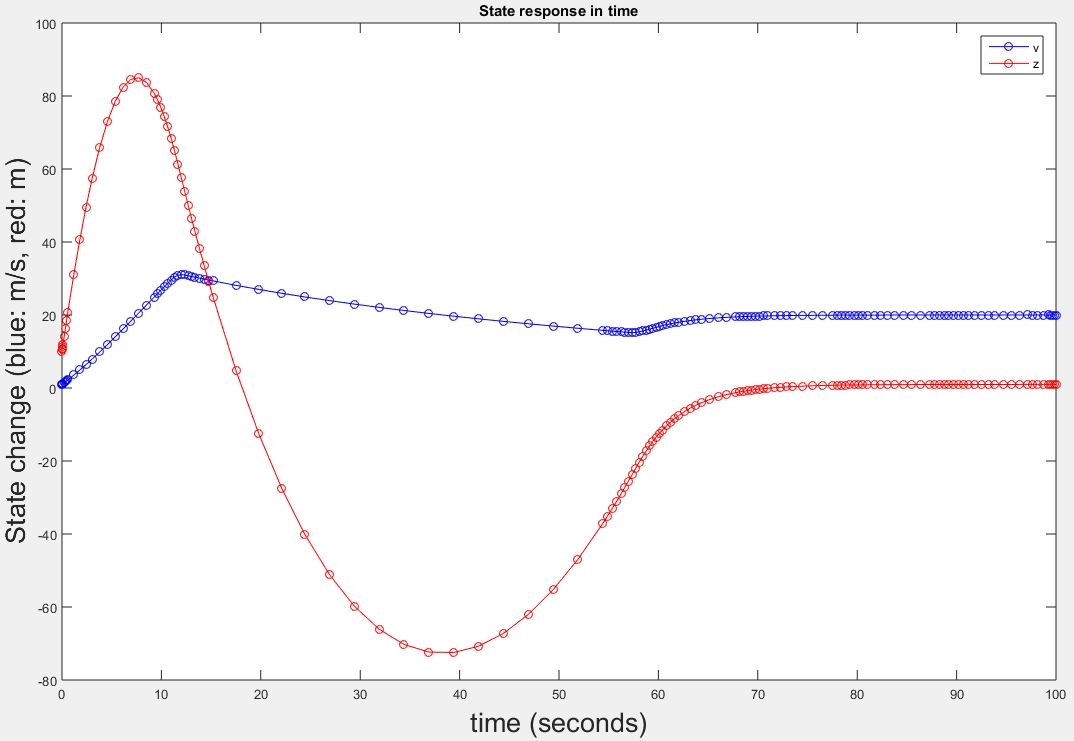
\includegraphics[width=0.8\textwidth]{A2_state_time.jpg}
\caption{States change in time}
\end{figure}
\end{center}

\clearpage

Below are several views of the corresponding phase portrait; with different levels of zoom to show the effect of the controller trying to reach a desired negative velocity (remember torque can only be positive, there is no reverse) which results in instability. In addition, there is a asymptotically stable equilibrium where V = Vr (= 20) and a corresponding integral state.


\begin{center}
\begin{figure}[htb]
	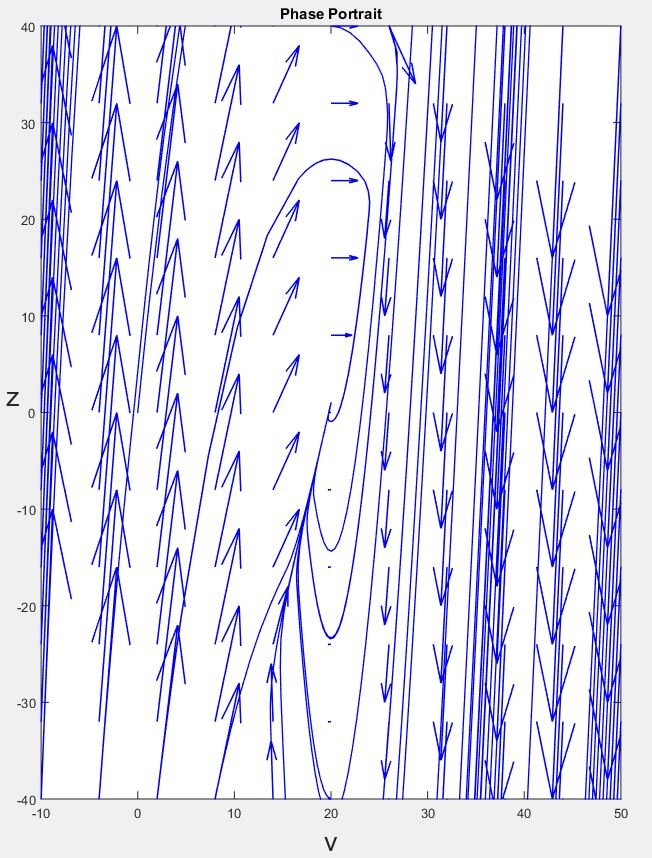
\includegraphics[width=0.6\textwidth]{A2_phaseportrait_1.jpg}
\caption{Phase Portrait of state variables v and z - note the stable equilibrium point at the regulated velocity}
\end{figure}
\end{center}


\clearpage

Zooming out further, it appears that the phase portrait represents a stable spiral for all initial conditions.


\begin{center}
\begin{figure}[htb]
	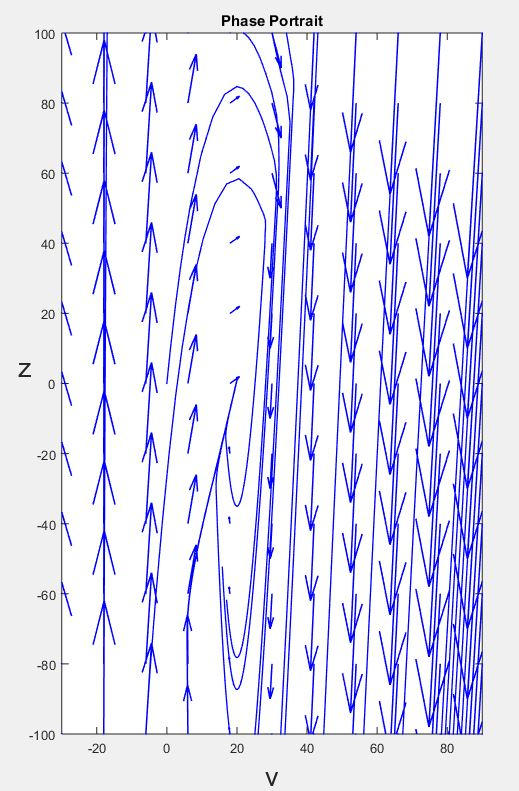
\includegraphics[width=0.6\textwidth]{A2_phaseportrait_2.jpg}
\caption{Phase Portrait of state variables v and z - note the stable equilibrium point at the regulated velocity}
\end{figure}
\end{center}

\clearpage

However, this is not true, it can be seen that for large velocities, where the angular velocity is exceeded for gear 3, it is indeterminable as to whether the trajectories return to the aforementioned equilibrium. This is shown in the figure below, which also shows that for negative velocities the system is unstable, as all initial conditions result in the two states growing with time.




\clearpage

\end{document}